\documentclass[letterpaper,12pt]{article}
\usepackage[top=3.0cm, bottom=3.0cm, left=3.0cm, right=3.0cm]{geometry}
\usepackage[spanish]{babel}
\spanishdecimal{.}
\selectlanguage{spanish}
\usepackage[spanish,onelanguage,ruled]{algorithm2e}
\usepackage[utf8]{inputenc}
\usepackage{graphicx}
\usepackage{caption}
\usepackage{subcaption}
\usepackage{hyperref}
\usepackage{verbatim}
\usepackage{amssymb}
\usepackage{mathtools}
\usepackage{amsmath}
\usepackage[natbibapa]{apacite}
\bibliographystyle{apacite}
%\usepackage[nottoc,numbib]{tocbibind}
\newcommand\ddfrac[2]{\frac{\displaystyle #1}{\displaystyle #2}}
\DeclareMathOperator{\atantwo}{atan2}
\title{Categoría AutoModelCar\\Torneo Mexicano de Robótica}
\author{Libro de Reglas, modalidad Virtual}
\date{Ciudad Victoria, 2022}

\begin{document}
\renewcommand{\tablename}{Tabla}
\maketitle

%%%%%%%%%%%%%%%%%%%%%%%%%%%%%%%%%%%%%%%
%%%%%%%%% AGRADECIMIENTOS %%%%%%%%%%%%%
%%%%%%%%%%%%%%%%%%%%%%%%%%%%%%%%%%%%%%%
\section*{Agradecimientos}
Esta competencia inició gracias al proyecto “Visiones de Movilidad Urbana” con el cual se dotó de 32 vehículos a escala a diferentes universidades, institutos y centros de investigación del país. Debido a la contingencia sanitaria, en 2021 se realizó por primera vez la modalidad virtual de esta competencia utilizando el simulador desarrollado por el equipo del Dr. Marco Morales del Instituto Tecnológico Autónomo de México. A nombre de todos los equipos que se han visto beneficiados, agradecemos a todos los académicos que han contribuido a la realización de esta competencia. 

\begin{flushright}
  \textit{
  El responsable técnico\\
  abril de 2022
  }
\end{flushright}


\section{Introducción}
El Torneo Mexicano de Robótica (TMR) es la competencia de robótica más importante de México que año con año reúne a estudiantes, profesores e investigadores. El objetivo principal es incentivar e impulsar la investigación y desarrollo de la robótica en México con miras a lograr un desarrollo integral de nivel internacional. Para lo anterior, el TMR incluye diferentes categorías de competición donde los equipos participantes ponen a prueba sus conocimientos y habilidades en la robótica.

Por segunda ocasión se abre la modalidad simulada de la categoría de vehículos sin conductor donde se proponen varias tareas de conducción autónoma. En la primera edición, se utilizó un simulador desarrollado para modelar los vehículos a escala AutoNOMOS, donados por la Universidad Libre de Berlín. Este año se utilizará el simulador Webots con el objetivo de tener vehículos y ambientes más parecidos a la realidad. 

Los antecedentes directos del presente libro de reglas son el evento realizado en el mes de abril de 2017 en el IPN en la ciudad de México y las ediciones anteriores de la categoría AutoModelCar del Torneo Mexicano de Robótica. El presente documento pretende tomar las pruebas propuestas con adecuaciones mínimas y establecer el criterio de competencia que fortalezca la participación académica y estudiantil, así como el intercambio de experiencias en pro del desarrollo y capacitación de profesionales en esta área del conocimiento.


%%%%%%%%%%%%%%%%%%%%%%%%%%%%%%%%%%%%%%%
%%%%%%%% SOBRE EL VEHÍCULO SIMULADO %%%%%%%%%%
%%%%%%%%%%%%%%%%%%%%%%%%%%%%%%%%%%%%%%%
\section{El vehículo simulado}

El simulador a utilizar es Webots\footnote{https://cyberbotics.com/doc/automobile/index} y el vehículos a utilizar es el modelo BMX X5\footnote{https://www.cyberbotics.com/doc/automobile/car?version=master} que ya incluye el mismo simulador. La figura \ref{fig:BmwX5} muestra la vista de este vehículo en el ambiente simulado. Este vehículo está equipado con los siguientes sensores:
\begin{enumerate}
\item Cámara RGB de 640x480 con 3\% de ruido. La cámara está colocada en la parte superior del parabrisas. 
\item Sensor Lidar 3D con las siguientes características:
  \begin{enumerate}
  \item Campo de vista horizontal: $360\deg$
  \item Campo de vista vertical: $18\deg$
  \item Número de capas: 32
  \item Distancia mínima: 0.01 m
  \item Distancia máxima: 75 m
  \item Resolución horizontal: 360
  \item Las demás establecidas en el simulador Webots\footnote{https://cyberbotics.com/doc/reference/lidar}.
  \end{enumerate}
\item GPS con resolución de 2m, ruido de 0.1m y las características por default del simulador Webots\footnote{https://cyberbotics.com/doc/reference/gps}
\item Giroscopio, con las características por default\footnote{https://www.cyberbotics.com/doc/reference/gyro?version=master}
\end{enumerate}

Se considera que las señales de control del vehículo son dos:
\begin{enumerate}
\item Velocidad lineal, dada en [m/s]
\item Ángulo de las llantas delanteras, en [rad]
\end{enumerate}
Es decir, no es necesario controlar el vehículos mediante pares o fuerzas, sino que el vehículo ya cuenta con un control para alcanzar las velocidades y ángulos deseados.

\begin{figure}
  \centering
  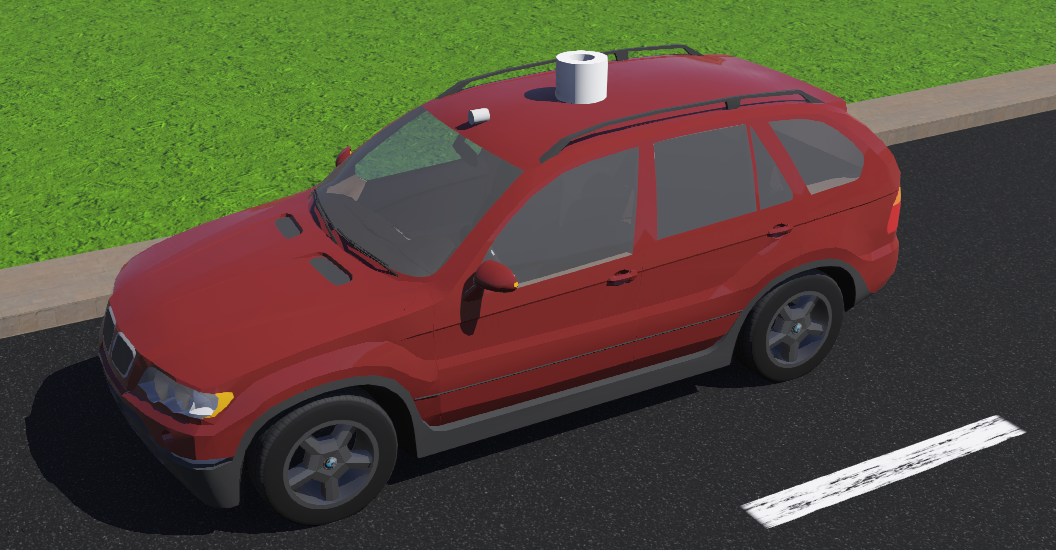
\includegraphics[width=0.75\textwidth]{Figures/Bmw.png}
  \caption{Vehículo simulado BMW X5}
  \label{fig:BmwX5}
\end{figure}

\subsection{Integración con ROS}
La modalidad virtual pretende ser lo más parecido posible a la modalidad presencial. Con esta idea, el vehículo simulado está integrado con ROS de modo que el software desarrollado para los vehículos reales pueda servir en el simulador. Por lo anterior, la forma de interactuar con el vehículo simulado es mediante la publicación y suscripción de tópicos.

\begin{itemize}
\item Tópicos publicados:
  \begin{itemize}
  \item \texttt{/camera/rgb/raw} (sensor\_msgs/Image): Imagen RGB de la cámara
  \item \texttt{/point\_cloud} (sensor\_msgs/PointCloud2): Nube de puntos generada por el Lidar
  \item \texttt{/gps} (sensor\_msgs/NavSatFix): Lectura del GPS
  \item \texttt{/gyro} (sensor\_msgs/Imu): Lectura del giroscopio
  \end{itemize}
\item Tópicos suscritos:
  \begin{itemize}
  \item \texttt{/speed} (std\_msgs/Float64): Velocidad lineal deseada en [m/s]
  \item \texttt{/steering} (std\_msgs/Float64): Ángulo de las llantas delanteras en [rad]
  \end{itemize}
\end{itemize}

%%%%%%%%%%%%%%%%%%%%%%%%%%%%%%%%%%%%%%%
%%%%%%%% SOBRE LA ARENA  %%%%%%%%%%
%%%%%%%%%%%%%%%%%%%%%%%%%%%%%%%%%%%%%%%
\section{Sobre la arena}
\subsection{Pista de pruebas}
La pista de pruebas tiene proporciones similares a la pista utilizada en la modalidad presencial, aproximadamente 150 m de largo por 100 m de ancho. Consta de un circuito de doble carril (uno para cada sentido), con dos cruces y curvas de diferente radio de curvatura. La línea que divide los carriles es continua en las curvas y segmentada en las partes rectas. La figura \ref{fig:Pista} muestra la pista simulada. 
\begin{figure}
  \centering
  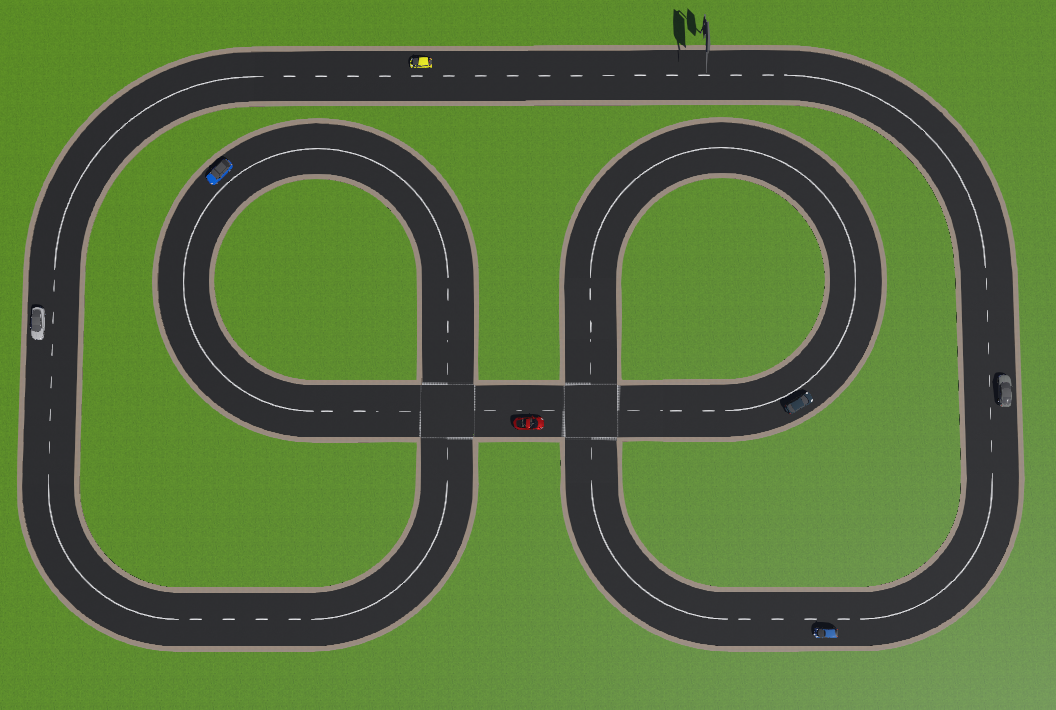
\includegraphics[width=0.75\textwidth]{Figures/Pista.png}
  \caption{Pista simulada}
  \label{fig:Pista}
\end{figure}

\subsection{Zona de estacionamiento}
Asimismo, habrá una zona separada de la pista para las pruebas de estacionamiento lateral. La figura \ref{fig:Parking} ilustra las dimensiones utilizadas para modalidad presencial. El espacio simulado tendrá proporciones similares, como se muestra en la figura \ref{fig:ParkingExample}. La banqueta será delimitada por “paredes” con altura suficiente para que pueda ser detectada por los sensores del robot. A diferencia de los años anteriores, el espacio para estacionarse estará delimitado por otros vehículos y no solo por paredes. Para este fin, se utilizarán otros vehículo simulados. 
\begin{figure}
  \centering
  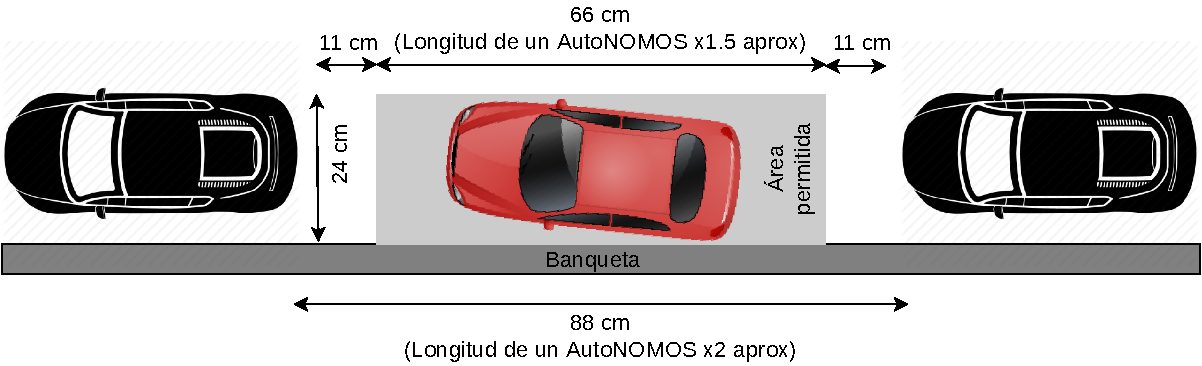
\includegraphics[width=0.95\textwidth]{Figures/Parking.pdf}
  \caption{Proporciones de la zona de estacionamiento}
  \label{fig:Parking}
\end{figure}

\begin{figure}
  \centering
  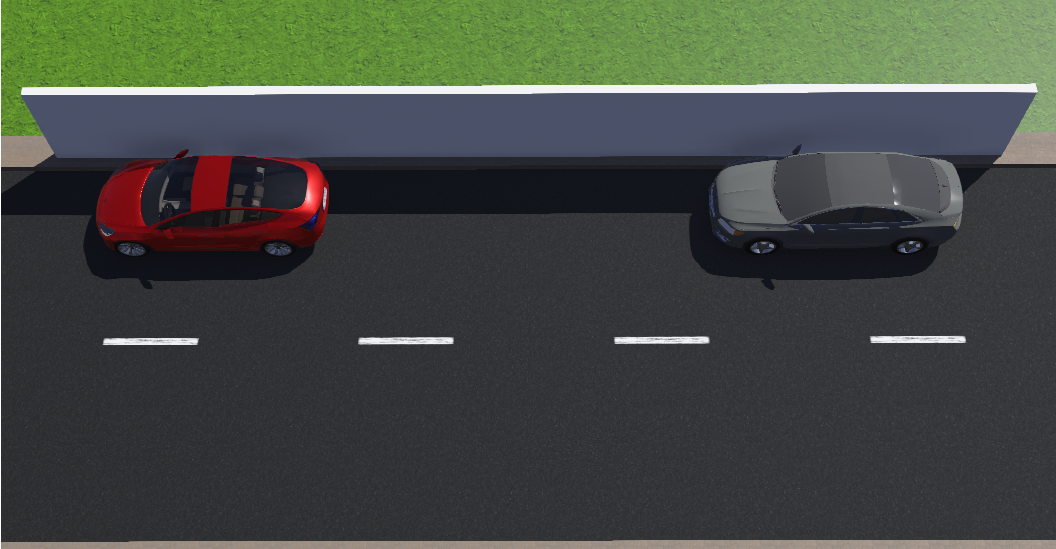
\includegraphics[width=0.95\textwidth]{Figures/ParkingExample.png}
  \caption{Zona de estacionamiento simulada}
  \label{fig:Parking}
\end{figure}


%%%%%%%%%%%%%%%%%%%%%%%%%%%%%%%%%%%%%%%
%%%%%%%%%%%%% REGLAS %%%%%%%%%%%%%%%%%%
%%%%%%%%%%%%%%%%%%%%%%%%%%%%%%%%%%%%%%%
\section{Reglas}
Todas las pruebas se llevarán a cabo dentro de la pista bajo las siguientes reglas:
\begin{enumerate}
\item Las pruebas se ejecutarán en la computadora destinada para este fin por el comité organizador. Niguna prueba se ejecutará en la computadora del equipo.

\item Cada equipo deberá subir su código a una rama del repositorio en GitHub (\url{https://github.com/mnegretev/TMR-2022-AutoModelCar}). A cada equipo registrado se le asignará una rama para que pueda subir su código.

\item En cada prueba se descargarán las actualizaciones hechas por el equipo y se ejecutarán. Es responsabilidad del equipo anunciar el procedimiento para la ejecución del código, el cual debe ser simple y preferentemente, con un solo comando.

\item Se realizarán tres intentos por prueba.

\item La pose inicial del automóvil (posición y dirección) será determinada por el comité técnico y podrá ser diferente para cada auto. Esta pose inicial se notificará al equipo en el momento de iniciar su prueba.

\item Si el automóvil participante choca contra algún objeto, persona, automóvil o ambientación dentro o fuera de la pista, la prueba se dará por terminada inmediatamente.

\item No se permiten modificaciones al ambiente de simulación.

\item \textbf{Aunque el simulador permite obtener la posición del vehículo en todo momento, esto no está permitido. La navegación autónoma deberá realizarse con base en la información disponible en los diferentes tópicos publicados por el simulador (cámara, lidar, gps, giroscopio).}
\end{enumerate}

%%%%%%%%%%%%%%%%%%%%%%%%%%%%%%%%%%%%%%%
%%%%%%%%%%%%% PRUEBAS %%%%%%%%%%%%%%%%%
%%%%%%%%%%%%%%%%%%%%%%%%%%%%%%%%%%%%%%%
\section{Pruebas}
Existen cuatro pruebas en el mismo circuito que implican diferentes niveles de dificultad:

\begin{enumerate}
\item \textbf{Navegación Autónoma sin Obstáculos.} Consiste en cubrir el circuito de inicio a fin sin abandonar el carril correspondiente.
\item \textbf{Navegación Autónoma con Obstáculos.} Consiste en cubrir el circuito con tres obstáculos estáticos en la pista. Estos obstáculos serán los vehículos de otros equipos colocados aleatoriamente a lo largo del circuito.
\item \textbf{Navegación Autónoma con Obstáculos en Movimiento.} Consiste en cubrir el circuito con dos obstáculos estáticos y uno móvil. El vehículo del equipo participante deberá ejecutar una maniobra de rebase en esta prueba. El obstáculo se moverá a una velocidad suficientemente baja para que el vehículo participante pueda ejecutar el rebase. Los otros dos obstáculos estarán colocados aleatoriamente a lo largo del circuito.
  \item \textbf{Estacionamiento Autónomo.} Consiste en hacer que el vehículo pueda estacionarse en la zona designada (ver figura \ref{fig:Parking}). Se arrancará el vehículo a un metro de distancia, aproximadamente, del espacio para estacionarse. La posición y orientación inicial tendrán una ligera variación aleatoria para todos los equipos. 
\end{enumerate}

Cada equipo tendrá 10 minutos para ejecutar cada prueba (o repetir las que desee). Durante este tiempo, el equipo participante podrá solicitar máximo 2 reinicios, para lo cual no se detendrá el cronómetro. Si el equipo no se encuentra listo al momento de que le corresponda
efectuar la prueba, la misma se dará por concluida sin puntos y pierde su turno. En este caso el tiempo restante se dará como tiempo de preparación para que el resto de los equipos puedan hacer una prueba rápida, mientras le toca el turno al siguiente equipo en la lista. Los equipos en la cola de espera deben estar listos para participar inmediatamente en cuanto les toque su turno. El orden de participación se realizará en forma aleatoria al inicio del concurso y éste debe ser respetado. Cada equipo debe participar en el turno que le corresponde.

\subsection{Presentación del póster}
Consiste en presentar un póster con la descripción del equipo, características del hardware, descripción de los métodos utilizados, resultados obtenidos y demás información que el equipo considere relevante. El cartel deberá tener un tamaño A1 y deberá ser presentado en el lugar y hora que el comité organizador designe al principio de la competencia.\textbf{La presentación del póster no otorga puntos pero es obligatoria para la participación en las demás pruebas}.

%%%%%%%%%%%%%%%%%%%%%%%%%%%%%%%%%%%%%%%
%%%%%%%PUNTUACIÓN Y DESEMPATE %%%%%%%%%
%%%%%%%%%%%%%%%%%%%%%%%%%%%%%%%%%%%%%%%
\section{Sistema de puntuación}
Los principios para establecer la puntuación que un equipo alcanza serán simples:
\begin{itemize}
\item Quien concluye el circuito exitosamente en las pruebas 1, 2 y 3, obtiene mayor puntuación que quien no lo termina.
\item Los equipos que concluyen exitosamente una prueba se ordenarán de acuerdo al tiempo que requirieron para cubrir el circuito, en orden ascendente.
\item Se aplicarán penalizaciones en forma de un tiempo predefinido (ver sección \ref{sec:penalties} sobre las sanciones) que se deberá sumar al tiempo total requerido por el equipo para concluir la prueba. 
\item El menor tiempo ganará la prueba.
\item Los equipos que no concluyen la prueba se ordenarán de acuerdo a la distancia del trayecto recorrido (durante un tiempo máximo de 5 minutos), restando 3 metros por cada minuto de sanciones acumulado. Por ejemplo, si alguien recorrió 9 metros en tres minutos y tiene un minuto de sanciones acumuladas se le asignará un recorrido total de 6 metros.
\item En la prueba sobre estacionamiento autónomo, se ordenará a los equipos de acuerdo al tiempo final requerido para concluir exitosamente la prueba, luego de aplicar sanciones a aquellos autos que colisionen contra algún obstáculo (ver sección \ref{sec:penalties}). Quien no logra estacionarse recibirá puntuación nula. Se considerará como exitosa la prueba si el vehículo queda estacionado dentro del espacio identificado en la Figura \ref{fig:Parking} como “Area permitida”.
\end{itemize}
\[\]
\[\]
\[\]
\subsection{Puntuación por prueba}
\label{sec:scoring}
Se otorgarán puntos por cada una de las pruebas de acuerdo a la posición ocupada en la lista de menores tiempos de acuerdo con la tabla \ref{tab:Scoring}. Si un equipo no participa en una prueba, obtendrá cero puntos en la misma.

\begin{table}[h!] 
  \centering
  \begin{tabular}{|c|c|c|c|c|c|c|c|c|c|c|}
    \hline
    Lugar &    1&   2&   3&   4&   5&   6&   7&   8&   9&10\\
    \hline
    Puntos & 50 & 45 & 40 & 35 & 30 & 25 & 20 & 15 & 10 & 5\\
    \hline
  \end{tabular}
  \caption{Puntuación por prueba}
  \label{tab:Scoring}
\end{table}


\subsection{Sanciones}
\label{sec:penalties}
A continuación se detalla la lista de causas y penalizaciones en tiempo:
\begin{table}[h!]
  \centering
  \begin{tabular}{|p{0.65\textwidth}|p{0.3\textwidth}|}
    \hline
    $\qquad\qquad$Causa & Penalización\\
    \hline
    Salir del carril parcialmente, regresando en menos de 5 segundos. & 5 segundos\\
    \hline
    Salir completamente del carril, regresando en menos de 5 segundos & 10 segundos\\
    \hline
    Salir (total o parcialmente) y tardar más de 5 segundos en regresar al carril. & 20 segundos\\
    \hline
    Tocar un obstáculo estático o móvil. & 30 segundos\\
    \hline
    Salir del carril (total o parcialmente) y no regresar en 30 segundos.  & 30 segundos y conclusión de la prueba.\\
    \hline
    Tocar un obstáculo durante la prueba de estacionamiento. & 10 segundos\\
    \hline
  \end{tabular}
  \caption{Penalizaciones}
  \label{tab:Penalties}
\end{table}

\subsection{Puntuación Final}
\label{sec:final_score}
Los puntos obtenidos en cada prueba se multiplicarán por un factor de ponderación asociado a cada prueba, como se indica en la tabla \ref{tab:weights}. La puntuación total será la suma de cada prueba por su factor de ponderación.

\begin{table}[h!]
  \centering
  \begin{tabular}{|l|c|}
    \hline
    Prueba & Factor de ponderación\\
    \hline
    Navegación sin obstáculos & 1.0 \\
    \hline
    Navegación con obstáculos estáticos & 1.5 \\
    \hline
    Navegación con obstáculos en movimiento & 2.0 \\
    \hline
    Estacionamiento\\
    \hline
  \end{tabular}
  \caption{Factores de ponderación por prueba}
  \label{tab:weights}
\end{table}


\subsection{Criterios de desempate}
En el caso del primer, segundo y tercer lugares generales de la categoría, se tomará como primer criterio de desempate designar como ganador a aquel que tenga la mayor suma de factores de peso de las pruebas donde participó obteniendo puntuaciones mayores a cero, es decir, en función del grado de dificultad de las pruebas en las que participó.

Si el empate aún persiste, el segundo criterio de desempate será designar como ganador al equipo que recibió el menor número de penalizaciones (sumando las penalizaciones totales). Si el empate aún persiste, el tercer criterio de desempate será el número de pruebas individuales en las que se participó y se obtuvo puntuación positiva.

Si el empate persiste después de aplicar los criterios anteriores, se acreditará el mismo lugar a los equipos que se mantengan en la misma posición y se declararán vacantes los lugares que ocuparían en caso de que no hubiera empate.

%%%%%%%%%%%%%%%%%%%%%%%%%%%%%%%%%%%%%%%
%%%%%%%%%% CONTACTO %%%%%%%%%%%%%%%%%%%
%%%%%%%%%%%%%%%%%%%%%%%%%%%%%%%%%%%%%%%
\section{Contacto}
Cualquier duda o aclaración favor de dirigirla vía email a:

Dr. Marco Negrete \texttt{marco.negrete@ingenieria.unam.edu}


%%%%%%%%%%%%%%%%%%%%%%%%%%%%%%%%%%%%%%%
%%%%%%%%% CRÉDITOS %%%%%%%%%%%%%%%%%%%%
%%%%%%%%%%%%%%%%%%%%%%%%%%%%%%%%%%%%%%%
\section*{Créditos}
El formato, textos y estructura del presente documento se basó en el reglamento para la categoría de drones del Torneo Mexicano de Robótica 2017 elaborado por el Dr. José Martínez Carranza y el Dr. Enrique Sucar Succar, y en los reglamentos de ediciones anteriores de esta misma competencia. 
\end{document}


\end{document}



